\documentclass[11pt]{article}

\usepackage{graphicx}
\usepackage{amsmath}
\usepackage{mathtools}
\usepackage{amsfonts}
\usepackage{fullpage}
%\usepackage{subfigure}
\usepackage{fancyvrb}
\usepackage{lipsum}
\usepackage{multirow}

\usepackage[ruled,vlined]{algorithm2e}

\newcommand{\ud}{\,\mathrm{d}}
\newcommand{\argmax}{\operatornamewithlimits{argmax}}

\title{Practical optimal experiment design for psychology}
\author{Daniel L. Ly, Long Ouyang, Daniel J. Hawthorne, Noah D. Goodman}
\date{}
%\nodate

\begin{document}

\maketitle

\begin{abstract}
\lipsum[1]
\end{abstract}

\section{Introduction}
    \begin{itemize}
        \item It is often difficult to discriminate between models of psychological processes
        \item Model analysis can be challenging and experiments can be expensive
        \item This paper presents a general and turn-key approach to design experiments that best disambiguates competing models using a Bayesian framework
        \item This technique is not directly related to Bayesian models of cognition. It can be used on any probabilistic model, including Bayesian models of cognition
        \item Despite the previous work in this field, there are a number of pragmatic issues that make it difficult to readily apply OED techniques for psychology, including:
        \begin{itemize}
            \item A variety of proposed optimization criteria, which puts the burden on researchers to have sufficient expertise to select the appropriate approach
            \item A lack of an established pipeline, requiring researchers to develop a language to formalize psychological models and write an OED optimization engine
            \item A lack of analysis in dealing with practical experimental concerns such as:
                \begin{itemize}
                    \item Noisy responses from participants
                    \item The ideal number of participants for a study
                    \item The ambiguity of linking functions of dependent measures
                \end{itemize}
        \end{itemize}
        \item \emph{Todo: breakdown of the paper with case studies}
    \end{itemize}

\section{Related work}
    \begin{itemize}
        \item OED has a long history in statistics and control systems
            \begin{itemize}
                \item Although much of the underlying theory is related, OED for practical psychology presents a variety of challenges that are not addressed by this work
            \end{itemize}
        \item There is related work on adaptive experiment design to find psychometric thresholds
            \begin{itemize}
                \item This work generally focuses on lower level psychophysics, while our approach is targeted towards higher level cognitive models
            \end{itemize}
        \item Myung and Pitt developed an approach for OED to discriminate psychological models
            \begin{itemize}
                \item Their approach maximizes the degree of model dissimilarity according to a utility function that quantifies a badness-of-fit measure
                \item Primary differences between our approaches:
                    \begin{itemize}
                        \item Their choice of utility functions is individually tailored to each problem, whereas we present a general framework 
                        \item Our OED approach explicitly differentiates between parameterized models and classes of models with internal parameters
                        \item We demonstrate a closed-loop process with empirical data and analysis gathered using Mechanical Turk
                        \item The single framework allows for mathematical analysis on considerations such as the number of subjects and designing joint sets of experiments
                    \end{itemize}
            \end{itemize}
    \end{itemize}

\section{Bayesian Model Selection Framework}
\label{s:bayes}

In this section, we describe the mathematical and theoretical framework of our OED approach in greater detail. Although this section is intended to provide readers with a rigorous and formal foundation for understanding the principles behind our approach, an open source computational implementation is readily available for those who are interested in applying our experiment design approach to their own models (REF). This section provides a preliminary overview of the general mathematic concepts, with additional theoretical analysis in Sections~\ref{s:class:ss:math} and \ref{s:npart:ss:math}, which examines the role of model parameterization and the number of participants, respectively.

The purpose of our OED approach is to quantitatively measure the ability of an experiment at differentiating competing computational models. Our approach leverages Bayesian inference, a powerful statistical technique, to reason about the uncertainty of which model best describes a given phenomenon. By using the models' predictions to compute the likelihood of observing a particular response to an experiment, this approach provides a rational method for updating the change in belief about model uncertainty when such responses are observed. This change in belief is then quantified using information theoretic measures, and by maximizing these measures, OED allows one to find experiments that should maximally change the uncertainty of the beliefs in our models. 

Before applying experiment design, one must define the experiment design space as well as the set of candidate models to be distinguished. The experiment design space characterizes the set of all design considerations that can be directly manipulated by the experimenter to generate distinct experimental prompts. Next, the experimenter must define a set of formal models that can predict the likelihood of observing a response for each experiment prompt. 

More formally, for a set of experimental prompts, $\mathcal{X}$, let the choice of experiment be defined as $x \in \mathcal{X}$. Similarly, for a set of responses, $\mathcal{Y}$, let $Y_x \in \mathcal{Y}$ be a random variable that describes the distribution over the possible outcomes of the experiment $x$. Also, for a set of candidate models, $\mathcal{M}$, let $M \in \mathcal{M}$ be a random variable that describes the uncertainty over which model best represents the underlying phenomenon of interest. Each model defines a stochastic relationship between prompts and responses. For a given model $m$, let the probability of observing an outcome $y$ given a prompt $x$ be defined as $x \rightarrow Y_x: P(Y_x = y_x | M = m)$.

As a brief aside on notation, we will use upper case symbols to represent random variables and lower case symbols to represent their corresponding realizations. For brevity, the probability of observing a particular realization will often be written without the random variable and using only the lower case symbol -- $p(y_x|m)$ represents $P(Y_x = y_x | M = m)$.

As there is a collection of candidate models, the goal of OED is to reason over the uncertainty of which model best represents the underlying phenomenon of interest. This uncertainty is quantified as a probability distribution, $p(m)$. This distribution is often referred to as the \emph{prior model belief distribution} as it expresses the uncertainty before any experiment design can be taken into account. The choice of this distribution is another design decision of the experimenter. Uninformative priors, such as assuming that all candidate models are equally plausible, are popular starting points. However, non-uniform priors, which relatively favor a particular subset of models, are also suitable if prior knowledge about the domain, such as previously collected data or established literature, can be leveraged. 

The next step is to consider how the model belief distribution should change as a result of observing a response, which is often referred to as the \emph{posterior model belief distribution}. Using Bayes' theorem, the uncertainty of the model $m$ after observing the response $y_x$ is defined as:
\begin{align}
p(m|y_x) = \frac{p(y_x|m)p(m)}{\sum\limits_{m'} p(y_x|m')p(m')}. \label{eq:bayes}
\end{align}
This fundamental formulation allows for the computation of the posterior, $p(m|y_x)$, solely as a function of the model predictions, $p(y_x|m)$, and the prior, $p(m)$.

The efficacy of an experiment is defined by its ability to differentiate between the candidate models, or equivalently, induce a change in the model belief. This approach is quantified using the Kullback-Liebler divergence (KL divergence), a non-symmetric relative measure between two probability distributions, to compute the information gain between the posterior and prior distributions for a given prompt:
\begin{align}
D_{\text{KL}}\left(p(m|y_x) || p(m)\right) = \sum\limits_m p(m|y_x) \ln \left( \frac{p(m|y_x)}{p(m)}\right). \label{eq:kl}
\end{align}
This measure computes the amount of extra information required to encode the posterior distribution using the prior distribution. If the two distributions of model beliefs are identical, then no additional information is required for the encoding and the information gain is zero, which concurs with the intuition that an experiment that did not change the model belief was useless. As the posterior and prior diverge, then information gain increases and the associated experiment is better at differentiating between the candidate models. For our framework, we use the natural logarithm, which corresponds to measuring information with the unit \emph{nats}. This choice was a matter of preference as logarithms with different bases, such as 2 or 10, are also popular choices. 

Although the previous analysis examined the information gain for a specific response, $y_x$, the full set of responses must be considered as the participants' reponses are not deterministic. Thus, the optimal experiment is the prompt $x^*$ that maximizes the expected KL divergence over the space of responses:
\begin{align}
x^* &= \argmax_{x} \sum\limits_{y_x} p(y_x) D_{\text{KL}}(p(m|y_x) || p(m)) \notag \\
    &= \argmax_{x} \sum\limits_{y_x} \left[\sum\limits_{m'} p(y_x|m')p(m')\right] D_{\text{KL}}(p(m|y_x) || p(m)). \label{eq:oed}
\end{align}
As Eq.~\ref{eq:kl} measures the information gain for a single response, taking the expected value of the KL divergence obtains the average information gain weighted by the probability of observing a response. This measure, Eq.~\ref{eq:oed}, defines the OED criteria as a function of only the experimental prompt. The probability of observing a result, $p(y_x)$, is computed by using its conditional probability definition, which leverages the model predictions, $p(y_x|m)$, and the prior, $p(m)$.

For the purposes of this paper, we will be focusing our analysis on the OED criteria of expected KL divergence and its properties, as opposed to the argument of the maximum component of the expression. Since Eq.~\ref{eq:oed} can rarely be solved analytically, it must be solved numerically which can often be a difficult task. To illustrate the advantages of our OED approach, we will be exhaustively evaluating the expected KL divergence for the entire prompt space. This allows us to obtain a comprehensive analysis of the entire design space and the challenge of selecting the optimal experiment is reduced to a simple sorting task. For large design spaces where exhaustive search is intractible, numerical optimization approaches, such as Sequential Monte Carlo searches (REF) or Bayesian optimization (REF), are viable options. 

It is worth noting that the expected KL divergence OED criteria, Eq.~\ref{eq:oed}, can be reformulated as the mutual information between the random variables for model belief, $M$, and response distribution, $Y_x$:
\begin{align}
x^* = \argmax_{x} \sum\limits_{y_x} p(y_x) D_{\text{KL}}(p(m|y_x) || p(m)) &= \argmax_{x} I(M, Y_x) \notag \\
    &= \argmax_{x} \sum\limits_{y_x} \sum\limits_{m} p(m, y_x) \ln \left( \frac{p(m, y_x)}{p(m)p(y_x)}\right). \label{eq:mi}
\end{align}
This reformulation uses a well-known identity between mutual information and the expected KL divergence~\cite{cover91:eit}. Mutual information is a measure of the amount of information one random variable contains about another, which provides an alternative perspective about the relationship between model belief and responses. This relationship, along with similar identities, will be useful for proving intrinsic properies about OED in Section~\ref{s:npart:ss:math}.

%    \begin{itemize}
%        \item For a space of prompts, $\mathcal{X}$, and a space of responses, $\mathcal{Y}$, let $x \in \mathcal{X}$ be the choice of experiment and $Y_x \in \mathcal{Y}$ be a random variable that describes the outcomes of the experiment $x$
%        \item For a collection of candidate models in the space $\mathcal{M}$, let $M \in \mathcal{M}$ be a random variable that describes the uncertainty over which model describes the underlying phenomenon of interest. Let $p(m)$ define a belief distribution that a specific model, $m$, describes the underlying phenomenon of interest 
%        \item Let the stochastic relationship between prompt $x$ and response $y$ for a given model $m$ be defined as $x \rightarrow Y_x: p(y_x|m)$
%        \item Upon observing an outcome of an experiment, the posterior belief distribution conditioned on observed data is defined as $p(m|y_x) = \frac{p(y_x|m)p(m)}{\sum_{m'} p(y_x|m')p(m')}$
%        \item Information gained from observing an outcome of an experiment is defined as the KL divergence between the prior and posterior belief distributions: $D_{KL}(p(m|y_x) || p(m)) = \sum_m p(m|y_x) \ln \left( \frac{p(m|y_x)}{p(m)}\right)$
%        \item The optimal experiment is the prompt $x^*$ that provides the maximum expected information gain: $x^* = \argmax_{x} \sum_y p(y_x) D_{KL}(p(m|y_x) || p(m))$
%        \item The expected information gain is equivalent to the mutual information between belief distributions and experiment responses: $I(M;Y_x) = D_{KL}(p(m,y_x)||p(m)p(y_x))$
%    \end{itemize}

\section{Case study 1: OED tutorial using probablistic programming languages}
\label{s:tutorial}

This section presents a tutorial on how to use optimal experiment design in conjuction with a probablistic programming language to disambiguate two models of subjective randomness. The case study begins with a short introduction to WebPPL, probabilistic programming language; followed by an example that illustrates the pipeline of formalizing cognitive models using WebPPL; and concludes with a summary of the OED analysis. 

\subsection{WebPPL -- a probabilistic programming language}

Probabilistic modelling is a powerful approach that is capable of quantifying degrees of belief using probabilities and allows for reasoning under uncertainty via probabilistic inference. Thus, it is no surprise that the use of probabilistic models has exploded in a variety of scientific domains where uncertainty is prevalent, including modern artificial intelligence, cognitive science, and applied statistics. However, as probabilistic models have become more sophisticated, the traditional tools for formal description and computation have wrestled with the increased complexity. Probabilistic programing languages (PPLs) provide a compositional approach for describing complex probability distributions and techniques for performing efficient probabilistic inference over an arbitrary program. 

In their simplest form, PPLs are extensions of a well-specified deterministic programming language with primitive constructs for random choice. Although the early forays in this field were explored in the 1980's, with foundational work by Giry, Kozen, Jones, Moggi, Saheb-Djahromi, Plotkin, and others~\cite{jones89:lics}, it has seen a resurgence due to new advances in probabilistic inference and the application-driven need for increased complexity. There are a wide range of recent probabilistic programming languages embodying different tradeoffs in expressivity, efficiency, and perspicuity~\cite{goodman08:uai, kimmig11:tplp, kiselyov09:dsl, maccallum09:nips, milch05:ijcai, pfeffer01:ijcai, pfeffer09:tr, poole08:pilp, richardson06:ml, sato97:ijcai}. 

If we view the semantics of the underlying deterministic language as a map from programs to executions of the program, the semantics of a PPL built on it will be a map from programs to distributions over executions. When the program halts with probability one, this induces a proper distribution over return values. Indeed, any computable distribution can be represented as the distribution induced by a Church program in this way~\cite{freer12:appl}.

WebPPL (pronounced `web people') is a probabilistic programming language built on top of a purely functional subset of Javascript. However, the functionality of WebPPL has been augmented with two critical features: the capacity to represent probability distributions and the ability to infer marginal distributions from arbitrary programs. First, probability distributions are represented using data structures called Elementary Random Primitives (ERPs). ERPs provide abstracted access to important features of probability distributions such as finding the support of the distribution, computing the log probability of each support, and sampling from the distribution. Although it is possible to define new ERPs directly, they are generally accessed using built-in primitive distributions or they are computed via inference functions. 

Second, WebPPL is equipped with a variety of implementations for probabilistic inference or marginalization: the operation of constructing the marginal distribution on return values. The ability for marginalization allows one to construct increasingly complex distributions in a compositional fashion. These marginalization functions take a random computation represented as an argumentless function and returns an ERP that captures the marginal distribution on return values. A variety of inference operators has been implemented in WebPPL, including enumeration, Metropolis-Hastings~\cite{metropolis53:jcp, hastings70:bio} and Particle Filters~\cite{gordon93:rsp, liu98:jasm}. 

To illustrate the use of WebPPL, consider computing the probability distribution from a single coin toss when three fair coins are tossed and at least two coin tosses come up heads. The traditional approach for computing this probability distribution requires the manual construction the conditional probability table that lists each event and its associated probability, followed by marginalizing over the subset of events that satisfy the precondition. Although this approach is suitable for simple distributions, scaling to arbitrary complex models can be challenging. Instead, WebPPL provides a formal language to construct compositional probability distributions.

\begin{figure}[h]
\begin{Verbatim}[numbers=left,numbersep=1pt,frame=single,commandchars=\\\{\},fontfamily=courier,fontsize=\scriptsize]
var atleast_two_heads = function() \{
  var coin_0 = sample(bernoulliERP, [0.5]); \label{ln:webppl_ex_coin0}
  var coin_1 = sample(bernoulliERP, [0.5]);
  var coin_2 = sample(bernoulliERP, [0.5]); \label{ln:webppl_ex_coin2}
  var sum_coins = coin_0 + coin_1 + coin_2;
  factor((sum_coins >= 2) ? 0 : -Infinity);
  return coin_0;
\}

var atleast_two_heads_erp = Enumerate(atleast_two_heads)
\end{Verbatim}
\centering
\caption{A WebPPL program to compute the probability distribution from a single coin toss when three fair coins are tossed and at least two coin tosses come up heads.}
\label{fig:webppl_intro}
\end{figure}

The WebPPL program for the coin toss example is shown in Fig.~\ref{fig:webppl_intro}. We define an argumentless function, \texttt{atleast\_two\_heads}, that encapsulates the computation of interest. The program is constructed by composing generative models with computation. First, three fair coins are sampled from a Bernoulli distribution with a success parameter of 0.5. The number of heads events are computed by summing up the three coin flip random variables. The \texttt{factor} keyword is then used to re-weight the log probability of an event occuring -- in this scenario, the situation where there are not at least two heads events is disregarded by assigning a zero probability to these outcomes, and the probability for the remaining outcomes is otherwise unaffected. Finally, the outcome of the first coin is returned. 

The \texttt{Enumerate} function is called to compute the marginal distribution of \texttt{alteast\_two\_heads} by exploring the executions of the random computation. The inference function returns an ERP that summarizes the probability distribution the coin toss. The ERP has a support of two outcomes, `0' and `1', which represents the tails and heads outcomes respectively, as well as the probabilities of each event, 1/4 and 3/4, respectively. This agrees with our basic intuitions as there are four outcomes where three coin tosses result in at least two heads events and, of these outcomes, there is only one where a specific coin can have a tails event.

The upcoming sections will further illustrate how to build increasingly complex probabilistic models using this basic framework of constructing probability distributions by composing generative models with computation (Section~\ref{s:tutorial:ss:randomness}).

\subsection{Models of subjective randomness}
\label{s:tutorial:ss:randomness}
People's judgements about randomness are frequently misunderstood -- for example, a sequence of heads and tails such as `HTHTTTHH' is often considered to be more random than the sequence `HHHHHHHH'. Although we have strong intuitions regarding the randomness of these sequences, both sequences are actually equally likely to be produced from flipping a fair coin. In fact, there is strong evidence that people have compelling preferences for certain sequences when considering random processes ~\cite{goodfellow38:jep}. The apparent discreptancy between our intuitions about randomness has garnered significant attention from both the mathematical~\cite{chaitin01:er, kac83:as, li97:kca} and psychological~\cite{falk81:pme, lopes82:jep, griffiths01:cogsci} literature. 

In this case study, we consider two models of randomness judgements: independent flips from a biased coin and a sequence of flips from a Markov chain. These models are not expected to fully characterize the observed intricacies of human judgements about randomness, but they provide a practical case study for understanding how optimal experiment design can be used to differentiate competing models. 

For this scenario, the participants will be prompted to judge the randomness of a four flip coin sequence by reporting the whether the next flip from the same coin will come up heads. Following the formalization outlined in Section~\ref{s:bayes}, the space of subjective randomness models under consideration is $\mathcal{M} \in \{m_b, m_m\}$, where $m_b$ and $m_m$ correspond to the biased coin model and the Markov coin model, respectively. The space of experimental prompts, $\mathcal{X}$, is the set of all four flip coin sequences, and the space of responses, $\mathcal{Y}$, is a choice between heads or tails.

\subsubsection{Biased coin model}
\label{s:tutorial:sss:biased}

The first model of subjective randomness is a biased coin model, which assumes that the coin is weighted with an unknown bias and each coin flip is independent. The coin bias is inferred from the experiment prompt sequence, and it is subsequently used to predict the next coin flip. The model will be formalized mathematically and in WebPPL to illustrate how one can translate a model between both frameworks.

We begin with the generative model of the biased coin model, which follows a Bernoulli distribution with an unknown bias parameter. Let the random variable $X$ represent the probability of observing the outcome of a coin flip, where the flip outcome can take on two values, $x \in \{\textrm{H},\textrm{T}\}$, representing heads or tails, respectively. Next, let the random variable $\Theta_b$ represent the uncertainty of the coin bias, where the bias parameter, $\theta_b \in [0,1]$, denotes the probability of a heads outcome. The probability of observing a coin flip outcome is then defined conditionally with respect to the bias parameter as:
\begin{align}
    P(X = \textrm{H} | \Theta_b = \theta_b) &= \theta_b \notag \\ 
    P(X = \textrm{T} | \Theta_b = \theta_b) &= 1 - \theta_b \label{eq:bcoin_x}.
\end{align}
Assuming that the experiment response, $Y$, is drawn from the same coin, the probability of observing a response given the bias parameter is similarly defined as: 
\begin{align}
    P(Y = \textrm{H} | \Theta_b = \theta_b) &= \theta_b \notag \\ 
    P(Y = \textrm{T} | \Theta_b = \theta_b) &= 1 - \theta_b \label{eq:bcoin_y}.
\end{align}

The coin bias, $\Theta_b$, is inferred from the experiment prompt, which is an $n$-length coin flip sequence, $x_0, x_1, \dots, x_n$. Applying Bayes theorem along with a prior distribution over the bias parameter, $p(\theta_b)$, the distribution of the bias parameter can be computed using:
\begin{align}
    p(\theta_b | x_0, x_1, \dots, x_n) &= \frac{p(x_0,x_1, \dots, x_n | \theta_b)p(\theta_b)} {\sum\limits_{\theta'_b} p(x_0, x_1, \dots, x_n | \theta'_b)p(\theta'_b)} \label{eq:bcoin_bayes}.
\end{align}

Using the property that each observation is an identical and independent sample from the generative biased coin, Eq.~\ref{eq:bcoin_bayes} can be decomposed into its elementary terms:
\begin{align}
    p(\theta_b | x_0, x_1, \dots, x_n) &= \frac{p(x_0 | \theta_b) p(x_1 | \theta_b) \dots p(x_n | \theta_b) p(\theta_b)} {\sum\limits_{\theta '_b} p(x_0 | \theta'_b) p(x_1 | \theta'_b) \dots p(x_n | \theta'_b) p(\theta'_b)} \label{eq:bcoin_iid},
\end{align}
where the probability $p(x_i | \theta_b)$ is given by Eq.~\ref{eq:bcoin_x}.

Finally, the probability of observing a model response for the biased coin model can be computed using:
\begin{align}
    p(y_{x_0 x_1 \dots x_n} | m_b) = \sum \limits_{\theta_b} p(y | \theta_b) p(\theta_b |  x_0, x_1, \dots, x_n),
\end{align}
where the probabilities $p(y | \theta_b)$ and $p(\theta_b | x_0, x_1, \dots, x_n)$ are given by Eqs.~\ref{eq:bcoin_y} and~\ref{eq:bcoin_iid}, respectively. 

\begin{figure}[h]
\begin{Verbatim}[numbers=left,numbersep=1pt,frame=single,commandchars=\\\{\},fontfamily=courier,fontsize=\scriptsize]
// Helper functions and model parameters \label{ln:wbc_help_s}
var categorical = function(v,p) {return v[discrete(p)];}
var coin_prior     = [0.01, 0.1, 0.2, 0.3, 0.4, 0.5, 0.6, 0.7, 0.8, 0.9, 0.99];
var coin_prior_pmf = [1.00, 1.0, 1.0, 1.0, 1.0, 1.0, 1.0, 1.0, 1.0, 1.0, 1.00]; \label{ln:wbc_help_e}

// Bias coin model
var bias_coin_erp = function(sequence) \{
  var bias_coin = function() \{
    var inferred_bias_erp = Enumerate(function() \{ \label{ln:wbc_infer_s}
      var bias_p = categorical(coin_prior, coin_prior_pmf); 
      var sequence_factor = sum(map(function(x) \{
                                      return (x == 'H') ? Math.log(bias_p) : 
                                                          Math.log(1-bias_p);\}, 
                                sequence));
      factor(sequence_factor);
      return bias_p;
    \}); \label{ln:wbc_infer_e}

    var bias_p = sample(inferred_bias_erp); \label{ln:wbc_sample}
    return flip(bias_p); \label{ln:wbc_flip}
  \};

  return Enumerate(bias_coin); \label{ln:wbc_enum}
\};
\end{Verbatim}
\centering
\caption{A WebPPL code snippet that models the randomness judgement from the biased coin model given a coin sequence.}
\label{fig:webppl_biased_coin}
\end{figure}

The WebPPL program for the biased coin model is shown in Fig.~\ref{fig:webppl_biased_coin}. The program begins with defining general utility code (lines~\ref{ln:wbc_help_s}-\ref{ln:wbc_help_e}): a helper function for sampling from a categorical distribution and the manual definition of the model parameter prior distributions, which are assumed to be uninformative prior or the uniform distribution. 

Following a similar progression as the mathemetical model, the WebPPL biased coin model first infers the bias coin parameter from the experiment prompt coin sequence (lines~\ref{ln:wbc_infer_s}-\ref{ln:wbc_infer_e}). A random bias parameter is sampled from the prior distribution, and is used to compute the probability of observing the coin flip sequence given the sampled prior distribution. An bias parameter is then sampled from the marginal distribution conditioned on the coin sequence (line \ref{ln:wbc_sample}) and a response of heads or tails is computed by flipping a random coin based on the sampled bias parameter (line \ref{ln:wbc_flip}). The distribution of responses is computed by enumerating over the space of responses (line \ref{ln:wbc_enum}). Note how the complexity of the mathemtical model of the biased coin model be readily described using WebPPL via composition of generative models and probabilistic inference. 

\subsubsection{Markov coin model}
\label{s:tutorial:sss:markov}
The second model of subjective randomness is a Markov coin model, which assumes that the coin is generated by a Markov process where each coin flip depends on the previous coin flip. The probability of transitioning from the current coin flip is inferred from the experiment prompt sequence, and it is subsequently used to predict the next coin flip. Again, the model will be formalized mathematically and in WebPPL to illustrate how one can translate a model between both frameworks.

We begin with the generative model of a two state Markov process, where the system is characterized by states and the corresponding probability to transition between them. Let the sequence of random variables $X_1, X_2, \dots, X_n$ represent the probability of observing a sequence of coin flip outcomes, where each flip outcome can take on two values, $x_i \in \{H,T\}, \forall i \in \{0, \dots, n\}$, representing heads or tails, respectively. Next, let the random variable $\Theta_t$ represent the uncertainty of transitioning between coin flip outcomes, where the transition parameter, $\theta_t \in [0,1]$, denotes the probability that the current outcome is different than the previous outcome. The probability of observing a coin flip outcome is then defined conditionally with respect to the previous outcome and the bias parameter as:
\begin{align}
    P(X_i = \textrm{H} | X_{i-1} = \textrm{T}, \Theta_t = \theta_t) = P(X_i = \textrm{T} | X_{i-1} = \textrm{H}, \Theta_t = \theta_t) &= \theta_t \notag \\ 
    P(X_i = \textrm{H} | X_{i-1} = \textrm{H}, \Theta_t = \theta_t) = P(X_i = \textrm{T} | X_{i-1} = \textrm{T}, \Theta_t = \theta_t) &= 1 - \theta_t \label{eq:tcoin_x}.
\end{align}
Assuming that the experiment response, $Y$, is drawn from the same process, the probability of observing a response given the transition parameter is similarly defined using the last coin flip outcome as: 
\begin{align}
    P(Y = \textrm{H} | X_n = \textrm{T}, \Theta_t = \theta_t) = P(Y = \textrm{T}| X_n = \textrm{H}, \Theta_t = \theta_t) &= \theta_t \notag \\ 
    P(Y = \textrm{H} | X_n = \textrm{H}, \Theta_t = \theta_t) = P(Y = \textrm{T} | X_n = \textrm{T}, \Theta_t = \theta_t) &= 1 - \theta_t \label{eq:tcoin_y}.
\end{align}

The coin bias, $\Theta_t$, is inferred from the experiment prompt, which is an $n$-length coin flip sequence, $x_0, x_1, \dots, x_n$. Applying Bayes theorem along with a prior distribution over the transition parameter, $p(\theta_t)$, the distribution of the bias parameter can be computed using:
\begin{align}
    p(\theta_t | x_0, x_1, \dots, x_n) &= \frac{p(x_0, x_1, \dots, x_n | \theta_t)p(\theta_t)} {\sum\limits_{\theta'_t} p(x_0, x_1, \dots, x_n | \theta'_t)p(\theta'_t)} \label{eq:tcoin_bayes}.
\end{align}

Using the property that each observation comes from the Markov process, Eq.~\ref{eq:tcoin_bayes} can be simplified using conditional probabilities:
\begin{align}
    p(\theta_t | x_0, x_1, \dots x_n) &= \frac{p(x_1 | x_0, \theta_t) \dots p(x_n | x_{n-1}, \theta_t) p(\theta_b)} {\sum\limits_{\theta '_t} p(x_1 | x_0, \theta'_b) \dots p(x_n | x_{n-1}, \theta'_t) p(\theta'_t)} \label{eq:tcoin_markov},
\end{align}
where the probability $p(x_i | x_{i-1}, \theta_t)$ is given by Eq.~\ref{eq:tcoin_x}. Note that since the first outcome is observed and has no dependence, it is deterministic -- $p(x_0) = 1$.

Finally, the probability of observing a model response for the Markov coin model can be computed using: \begin{align}
    p(y_{x_0, x_1, \dots, x_n} | m_t) = \sum \limits_{\theta_t} p(y | x_n, \theta_t) p(\theta_t |  x_0, x_1, \dots, x_n),
\end{align}
where the probabilities $p(y | x_n, \theta_t)$ and $p(\theta_t | x_0, x_1, \dots, x_n)$ are given by Eqs.~\ref{eq:tcoin_y} and~\ref{eq:tcoin_markov}, respectively. 

\begin{figure}[h]
\begin{Verbatim}[numbers=left,numbersep=1pt,frame=single,commandchars=\\\{\},fontfamily=courier,fontsize=\scriptsize,firstnumber=last]
var markov_coin_erp = function(sequence) \{
  var markov_coin = function() \{
    var inferred_trans_erp = Enumerate(function() \{ \label{ln:wmc_infer_s}
      var trans_p = categorical(coin_prior, coin_prior_pmf);
      var sequence_factor = sum(map2(function(x,y) \{
                                       return (x == y) ? Math.log(1-trans_p) : 
                                                         Math.log(trans_p);\}, 
                                sequence.slice(0,sequence.length-1), 
                                sequence.slice(1,sequence.length)));
      factor(sequence_factor);
      return trans_p;
    \}); \label{ln:wmc_infer_e}

    var trans_p = sample(inferred_trans_erp); \label{ln:wmc_sample}
    return flip((last(sequence) == 'H') ? 1-trans_p : trans_p); \label{ln:wmc_flip}
  \};

  return Enumerate(markov_coin); \label{ln:wmc_enum}
\};
\end{Verbatim}
\centering
\caption{A WebPPL code snippet that models the randomness judgement from the Markov coin model given a coin sequence, continued from Fig.~\ref{fig:webppl_biased_coin}.}
\label{fig:webppl_markov_coin}
\end{figure}

The WebPPL program for the Markov coin model is shown in Fig.~\ref{fig:webppl_markov_coin}.  Following the framework of the mathemetical model, the WebPPL Markov coin model first infers the transition coin parameter from the experiment prompt coin sequence (lines~\ref{ln:wmc_infer_s}-\ref{ln:wmc_infer_e}). A random transition parameter is sampled from the prior distribution (Fig.~\ref{fig:webppl_biased_coin} lines~\ref{ln:wbc_help_s}-\ref{ln:wbc_help_e}), and is used to compute the probability of observing the coin flip sequence given the sampled prior distribution. A transition parameter is then sampled from the marginal distribution conditioned on the coin sequence (line \ref{ln:wmc_sample}) and a response of heads or tails is computed by flipping a random transition based on the sampled transition parameter and the last coin in the observed sequence (line \ref{ln:wmc_flip}). The distribution of responses is computed by enumerating over the space of responses (line \ref{ln:wmc_enum}). 

\subsection{Optimal experiment design}

The optimal experiment design execution in WebPPL is shown in Fig.~\ref{fig:webppl_oed}. First, the list of four flip coin sequences is manually enumerated. The \texttt{OED} function, which computes the argument of Eq.~\ref{eq:oed} for each of the experiments, is then called with an object that encapsulates the space of models and experiments. The two ERP-generating model functions, \texttt{bias\_coin\_erp} and \texttt{markov\_coin\_erp}, which were previously defined in Figs.~\ref{fig:webppl_biased_coin} and~\ref{fig:webppl_markov_coin}, respectively, are supplied in the object property \texttt{models}. Similarly, the list of arguments are supplied in the object property \texttt{experiments}. The model belief prior, $p(m)$, is supplied with the optional object property \texttt{model\_belief} as a list of probabilities that correspond to the model belief for each model. If no model belief distribution is specified, as in Fig.~\ref{fig:webppl_oed}, then it is assumed to be a uniform distribution. 

\begin{figure}[h]
\begin{Verbatim}[numbers=left,numbersep=1pt,frame=single,commandchars=\\\{\},fontfamily=courier,fontsize=\scriptsize,firstnumber=last]
// Execute the models and compute the information gain
var expt_list= ['HHHH', 'HHHT', 'HHTH', 'HHTT', 'HTHH', 'HTHT', 'HTTH', 'HTTT', 
                'THHH', 'THHT', 'THTH', 'THTT', 'TTHH', 'TTHT', 'TTTH', 'TTTT'];

var data = OED(\{models: [bias_coin_erp, markov_coin_erp], 
                experiments: expt_list\})
\end{Verbatim}
\centering
\caption{A WebPPL code snippet that calls the OED computational engine for the randomness judgement models, continued from Fig.~\ref{fig:webppl_markov_coin}.}
\label{fig:webppl_oed}
\end{figure}

\subsection{Results and discussion}

Executing the WebPPL code described in Figs.~\ref{fig:webppl_biased_coin}-\ref{fig:webppl_oed} returns a data structure that provides the information gain for each specified experiment. The results of executing experiment design for this randomness judgement case study is shown in Fig.~\ref{fig:coin}.

\begin{figure}[h!]
\centering
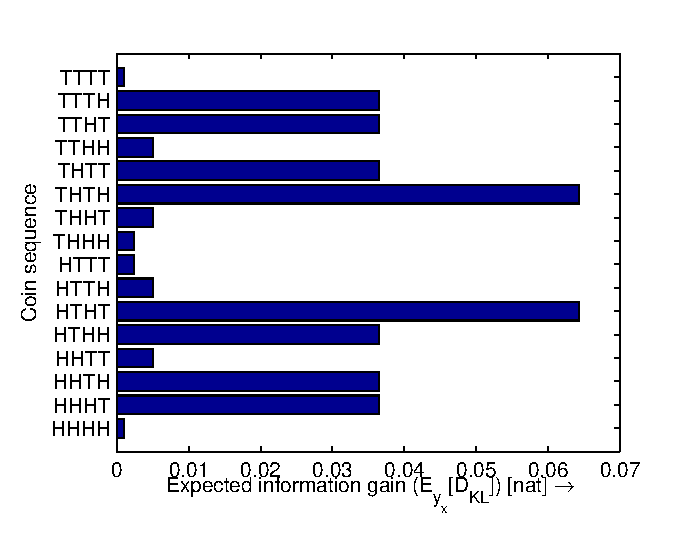
\includegraphics[width=3in]{img/coin.eps}
\caption{The information gain for all four flip coin sequences experiment prompts.}
\label{fig:coin}
\end{figure}

The results of the experiment design should be consistent with our intuitions about differentiating between the biased and Markov coin models. The most informative experiment prompts are the symmetric pair of coin sequences `HTHT' and `THTH'. The source of this information gain can be understood by analyzing the models independently. Using the `HTHT' coin sequence as an example, the bias coin observes two heads and two tails, infers that the bias should be centered around a fair weighting, and thus, does not favor either heads or tails as the next coin flip. In comparison, the Markov coin model infers that the flip sequence is alternating, and thus strongly favors the heads as the next coin flip in the sequence. By exploiting this difference in predictions, one can easily determine the underlying model from the response.

Following the same logic, the least informative experiment prompts are the symmetric pair of coin sequences `HHHH' and `TTTT'. Again, using the `HHHH' coin sequence as an example, the bias coin observes heads outcomes and thus infers that the coin is heavily biased towards heads outcome for the next coin. The Markov coin model infers that the flip sequence is unlikely to transition, and thus, also strongly favors a heads outcome for the next coin. Although each model has differing rationales for their predictions, they share the same prediction which makes it very difficult to determine the underlying model from an response. 

Furthermore, optimal experiment design is a powerful tool for obtaining general insights about both the experiment space and the candidate models. For example, the information gain is symmetric with respect to heads and tails symbol inversion. This should be expected as both models preserve their predictive distributions if the symbols are flipped. By observing general trends in the information gain of experiments, one can get a deeper understanding of the capabilities and limitations of the candidate models.

%    \begin{itemize}
%        \item Overview
%            \begin{itemize}
%                \item This case study is a toy example on disambiguating two models of subjective randomness
%                \item The purpose of this case study is to illustrate the pipeline of formalizing cognitive models using a probabilistic programming language and applying OED to find the optimal experiment
%            \end{itemize}
%        \item Models of subjective randomness
%            \begin{itemize}
%                \item We present two simple but plausible cognitive models of subjective randomness in the domain of random sequences
%                    \begin{enumerate}
%                        \item Independent flips from an identical coin
%                            \begin{itemize}
%                                \item Each event in the sequence is obtained from the same Bernoulli distribution
%                                \item The parameter of the Bernoulli distribution is inferred from the sequence
%                            \end{itemize}
%                        \item Flips from a Markov chain
%                            \begin{itemize}
%                                \item The sequence is generated from a Markov chain, where the outcome of an event depends on the previous event
%                                \item The transition parameter of the Markov chain is inferred from the sequence
%                            \end{itemize}
%                    \end{enumerate}
%                \item \emph{Include: graphical models of the two coin models}
%                \item \emph{Include: Church models of the two coin models}
%            \end{itemize}
%        \item Optimal experiment design
%            \begin{itemize}
%                \item We aim to present participants with a four event sequence and prompt them for the outcome of the next event
%                \item This is a simple experiment space with 16 possible prompts, which we exhaustively evaluate the information gain
%                \item \emph{Include: code example for invoking OED for this problem}
%            \end{itemize}
%        \item Results and discussion
%            \begin{itemize}
%                \item The optimal sequence is the symmetric pair of `0101' and '1010'
%                    \begin{itemize}
%                        \item The Markov model strongly predicts an alternating event, while the iid model does not favor either outcome
%                        \item The drastic difference between these predictions makes it easy to identify the underlying model
%                    \end{itemize}
%                \item The worst sequence is the symmetric pair of `0000' and '1111'
%                    \begin{itemize}
%                        \item Both models predict the same outcome, which is the repetition of the sequence
%                        \item As both models predict the same response, it is difficult to distinguish these models given this experiment prompt
%                    \end{itemize}
%                \item These results should agree with our intuitions about disambiguating these two models of subjective randomness
%                \item \emph{Include: plot of information gain for each sequence}
%            \end{itemize}
%    \end{itemize}

\section{Case study 2: Practical OED for classification learning with human participants}
\label{s:ms}

This section presents a real-world case study on how optimal experiment design can be used to differentiate competing models in the domain of classification learning. This case study builds on the classic experiment from Medin and Schaffer~\cite{medin78:pr}, and illustrates how computational approaches to experiment design can often outperform human intuition. In particular, this case study demonstrates the efficacy of OED in psychology for discrete and non-ordinal experiment spaces, large combinatoric experiment spaces, and parametric model classes. This section begins with a review of Medin and Schaffer's work on classification learning, followed by a description of the experiment design setup, and then concludes with analyzing empirical results from human participants obtained using Amazon's Mechanical Turk. 

\subsection{Models of Classification Learning}
The ability to form concepts and abstract rules is an integral component of cognitive science as it establishes a foundation for naming objects and events, as well as discussing and interacting with them. Since few concepts are formally taught, the formation and progression of classifying observations and experience into categories must be a fundamental learning phenomenon. As such, models of classification learning has been an active area of research in cognitive science for decades~\cite{machery10:bbs}. 

In this case study, we consider two formal models of classification learning: the Context Theory model and the Independent Cue model, which were the two models originally compared by Medin and Schaffer. These models were selected since they are well-known computational models that are well-suited for comparison described in a classic paper on classification learning. Furthermore, the authors describe their experiment design process in detail to explain how it is capable of differentiating the two candidate models, making this scenario ideal for evaluating whether automated experiment design approaches can outperform expert intuition. 

Following the experimental setup of Medin and Schaffer, participants are provided with exemplars from two categories and prompted to classify a set of stimuli individually (described in further detail in Section~\ref{ss:ms_setup}). The space of classification learning models under consideration is $\mathcal{M} \in \{m_{ct}, m_{ic}\}$, where $m_{ct}$ and $m_{ic}$ correspond to the Context Theory model and the Independent Cue model, respectively. The space of experimental prompts, $\mathcal{X}$, is the joint set of all possible training exemplars and probe stimuli, and the space of responses, $\mathcal{Y}$, is set the classifications of all the probe stimuli.

\subsubsection{Notation}

Before introducing the classification models, it is useful to discuss the notation for representing stimuli. The stimuli to be classified is represented as a composition of binary properties of four cue dimensions: color (red or blue), form (triangle or circle), size (large or small), and number (one or two). Each stimuli can be described using a binary code with `0' and `1' representing one of the properties, respectively. For example, using the dimension ordering of color, form, size and number, the notation `1001' might refer to a single small red circle, while `0110' would refer to a stimulus comprised of two large blue triangles. This binary code makes it easy to compare the similarity of stimuli: `1111' and `1101' differ only in size, while `0101' and `1101' differ only in color. 

\subsubsection{Context Theory Model}

The first classification model is the Context Theory model, which is built upon seven explicitly stated assumptions~\cite{medin78:pr}. For the purposes of computational experiment design, the two most relevant cognitive assumptions are that category judgements are based on the retrieval of exemplar information and that the overall similarity of two stimuli are comprised of multiplicative combinations between the similarity of retrival cues. These assumptions are formalized as a statistical model that uses a sum of product computation to determine the probability a stimulus will be associated with a given category.

Formally, let the variables $x_A$ and $x_B$ represent the sets of stimuli that correspond to exemplars in category A and category B, respectively. Furthermore, let the variable $x_s$ represent the set of stimuli that correspond to the probe stimuli, which is mutually exclusive with the category exemplars. Let the random variable $Y \in \{A,B\}^{|x_s|}$ represent the probability that each probe stimuli is classified to belong in a corresponding category. Let the variable $c_i$ represent the $i$th cue dimension and let the variable $w_i$ represent the corresponding model weighting parameter. The probability that the Context Theory model will classify the $k$th probe stimuli, $x_{sk}$, in the category $y_k$ is then defined as:
\begin{align}
    p(y_k | x_{sk}, x_A, x_B, w_1, \dots, w_d) &= \frac{\sum\limits_{x_j \in y_1} \prod\limits_{i=1}^d f_{ct}(x_{ski}, x_{ji}, w_i)}{\sum\limits_{c \in \{A,B\}}\sum\limits_{x_j \in c} \prod\limits_{i=1}^d f_{ct}(x_{ski}, x_{ji}, w_i)}, \label{eq:ct_base}
\end{align}
where $d$ is the size of the cue dimensions, and $f_{ct}$ is the similarity measure:
\begin{align}
    f_{ct}(x_{ski}, x_{ji}, w_i) = 
        \begin{dcases}
            1  , & \text{if } x_{ski} = x_{ji}\\
            w_i, & \text{otherwise}
        \end{dcases}.
\end{align}

\begin{figure}[h]
\hspace{1cm}
\begin{tabular}{ccccccccccc}
\multicolumn{5}{c}{Category A} & \hspace{1cm} & \multicolumn{5}{c}{Category B} \\
Stimulus & \multicolumn{4}{c}{Pattern} & & Stimulus & \multicolumn{4}{c}{Pattern} \\
  & $c_1$ & $c_2$ & $c_3$ & $c_4$ & & & $c_1$ & $c_2$ & $c_3$ & $c_4$  \\ \cline{2-5} \cline{8-11}
$s_1$ & 1 & 0 & 1 & 1 & & $s_4$ & 0 & 0 & 0 & 0 \\
$s_2$ & 1 & 1 & 1 & 0 & & $s_5$ & 0 & 0 & 1 & 1 \\
$s_3$ & 1 & 1 & 1 & 1 & & $s_6$ & 1 & 1 & 0 & 0 
\end{tabular}
\vspace{1cm}
\newline
\begin{tabular}{ccccc}
\multicolumn{5}{c}{Probe Stimuli} \\
Stimulus & \multicolumn{4}{c}{Pattern} \\
  & $c_1$ & $c_2$ & $c_3$ & $c_4$ \\ \cline{2-5} 
$s_7$ & 1 & 0 & 1 & 0 
\end{tabular}
\centering
\caption{An example set of stimuli for Category A, Category B, and probe stimuli.}
\label{fig:cat_example}
\end{figure}

To clarify the computation of Eq.~\ref{eq:ct_base}, consider the example shown in Fig.~\ref{fig:cat_example}. Using the provided set of stimuli, the probability that the probe stimulus will be classified in Category A is: 
\begin{align}
    p(A | x_s, x_A, x_B, w_1, \dots, w_d) 
        &= \frac{(1\!\cdot\!1\!\cdot\!1\!\cdot\!w_4) + (1\!\cdot\!w_2\!\cdot\!1\!\cdot\!1) + (1\!\cdot\!w_2\!\cdot\!1\!\cdot\!w_4)}{ \splitfrac{(1\!\cdot\!1\!\cdot\!1\!\cdot\!w_4) + (1\!\cdot\!w_2\!\cdot\!1\!\cdot\!1) + (1\!\cdot\!w_2 \cdot\!1\!\cdot\!w_4)}{+ (w_1\!\cdot\!1\!\cdot\!w_3\!\cdot\!1) + (w_1\!\cdot\!1\!\cdot\!1\!\cdot\!w_4) + (1\!\cdot w_2\!\cdot\!w_3\!\cdot\!1)}} \notag \\
        &= \frac{w_4 + w_2 + w_2w_4}{w_4 + w_2 + w_2w_4 + w_1w_3 + w_1w_4 + w_2w_3}. 
\end{align}
If all four parameters were equal to 0.3, then the probe stimulus $s_7$ should be classified in Category A with a probability of 0.72. 

As the model parameters are not a part of the experiment design, they must be marginalized out by using a prior distribution over the model parameter, $p(w_i)$:
\begin{align}
    p(y_k | x_{sk}, x_A, x_B) &=  p(y|x_{sk}, x_A, x_B ,w_1, \dots, w_n) p(w_1) \dots p(w_d),
\end{align}
which leverages the property that each model parameter, $w_i$, is independent.

Finally, the probability of classifying a set of probe stimuli for the Context Theory model is computed using: 
\begin{align}
    p(y_{1,\{x_{s1}, x_A, x_B\}}, \dots, y_{n,\{x_{sn}, x_A, x_B\}} | m_{ct}) &=  \prod\limits_{k=1}^{|x_s|} p(y_k|x_{sk}, x_A, x_B).
\end{align}

The WebPPL program for the Context Theory model is shown in Fig.~\ref{fig:webppl_ct}. TODO: The program begins with defining general utility code (lines~\ref{ln:wbc_help_s}-\ref{ln:wbc_help_e}): a helper function for sampling from a categorical distribution and the manual definition of the model parameter prior distributions, which are assumed to be uninformative prior or the uniform distribution. Talk about prior distributions. Talk briefly about the model. 


\subsubsection{Independent Cue Model}
The second classification model is the Independent Cue model, which assumes that the information entering category judgments can be derived from an additive combindation of the information from the component cue dimensions. Prototype, average distance and versions of cue validity and frequency models fall under this domain. This is a prototype model that classifies probe items by comparing similarities with a representative prototype of the category




Formally, let the variables $x_A$ and $x_B$ represent the sets of stimuli that correspond to exemplars in category A and category B, respectively. Furthermore, let the variable $x_s$ represent the set of stimuli that correspond to the probe stimuli, which is mutually exclusive with the category exemplars. Let the random variable $Y \in \{A,B\}^{|x_s|}$ represent the probability that each probe stimuli is classified to belong in a corresponding category. Let the variable $c_i$ represent the $i$th cue dimension and let the variable $w_i$ represent the corresponding model weighting parameter. The probability that the Context Theory model will classify the $k$th probe stimuli, $x_{sk}$, in the category $y_k$ is then defined as:

This is formalized as a rank-ordering model that uses an additive computation to determine the relative association with a given category

The first thing we need to consider is the information value and wthe associated weighting factor. When a pattern is presented to be classified at some point, the value associated witht eh color dimension will be sampled. If red is sampled, then the information would be positive since red is more closely associated with category A than B. If blue were sampled, then the information would be negative. This all depends on how informative each cue dimension is. Since this is all weighted anyways, we only really care about the relative information of each cue dimension, which we compute by computing the difference of positive examples over the total number of examples. The formulation is as follows:

\begin{align}
    f_{ic,A}(x_s, x_A, x_B, i) &= 
        \begin{dcases}
            \frac{\sum\limits_{x_a \in x_A} x_{ai} - \sum\limits_{x_b \in x_B} x_{bi}} {\sum\limits_{x_a \in x_A} x_{ai} + \sum\limits_{x_b \in x_B} x_{bi}}, & \text{if } x_{si} = 1 \\
            \frac{\sum\limits_{x_a \in x_A} (1-x_{ai}) - \sum\limits_{x_b \in x_B} (1-x_{bi})} {\sum\limits_{x_a \in x_A} (1-x_{ji}) + \sum\limits_{x_b \in x_B} (1-x_{bi})}, & \text{otherwise } 
        \end{dcases}
\end{align}

The good part of this formulation is that relective, where the information that a stimula is associated with catefory a is more likely to be associated with category b is simply the negative of each other:

\begin{align}
f_{ic,B}(x_s, x_A, x_B, i) = -f_{ic,A}(x_s, x_A, x_B, i)
\end{align}

Formulation into evidence? This gives a rank-ordering model.

To convert this rank-ordering model into a statistical one, we use a log-linear transformation to convert the relative associations into probabilities. Something about bayesian interpretation?

\begin{align}
    P(Y=A| x_s, x_A, x_B, w_0, w_1, \dots, w_d, \alpha) &= 
        \begin{dcases}
            \frac{1}{1 + e^{-\alpha \left(w_0 + \sum \limits_{i=1}^d w_i f_{ic,A}(y, x, i)\right)}}, & \text{if } x_s \in \{x_A \cup x_B\}\\
            \frac{1}{1 + e^{-\alpha \left(\sum \limits_{i=1}^d w_i f_{ic,A}(y, x, i)\right)}}, & \text{otherwise }
        \end{dcases}
\end{align}

$P(Y=B| x_s, x_A, x_B, w_0, w_1, \dots, w_d, \alpha) = 1- P(Y=A| x_s, x_A, x_B, w_0, w_1, \dots, w_d, \alpha)$, which arises from the property that $1-\frac{1}{1+e^{-x}} = \frac{1}{1+e^x}$, and $f_{ic,B}(x_s, x_A, x_B, i) = -f_{ic,A}(x_s, x_A, x_B, i)$.

Example.

\begin{align}
    p(y | x_s, x_A, x_B) &=  
        \begin{dcases}
            p(y|x_s, x_A, x_B, w_0, w_1, \dots, w_d, \alpha) p(w_0) p(w_1) \dots p(w_d) p(\alpha), & \text{if } x_s \in \{x_a \cup x_b\}\\
            p(y|x_s, x_A, x_B, w_1, \dots, w_d, \alpha) p(w_1) \dots p(w_d) p(\alpha), & \text{otherwise}
        \end{dcases}
\end{align}
since each $w_i$ is independent.

For a collection of stimuli, 
\begin{align}
    p(y_{1,\{x_{s1}, x_A, x_B\}}, \dots, y_{n,\{x_{sn}, x_A, x_B\}} | m_{ic}) &=  \prod\limits_{k=1}^n p(y_k|x_{sk}, x_A, x_B) 
\end{align}

code?

\subsection{Optimal Experiment Design}
With meticulous forethought, MS designed an experiment to disambiguate these two candidate models and then analyzed participant's performance on using this prompt. The prompt is shown in Fig. Explain the logic in their prompt.

Although MS provide sound arguments for their experiment design, does their experiment provide the optimal amount of information for disambiguating their competing models?

Constrained to the same MS experiment space, we exhaustively evaluated the 933 valid and unique experiments in terms of expected information gain

In particular, this case study demonstrates the efficacy of OED in psychology for discrete and non-ordinal experiment spaces, large combinatoric experiment spaces, and parametric model classes. 

\subsection{Results and Discussion}

MS is a suboptimal experiment that ranks in the 30$^\text{th}$ percentile with respect to expected information gain (Fig.~\ref{fig:dist})
\begin{figure}[h!]
\centering
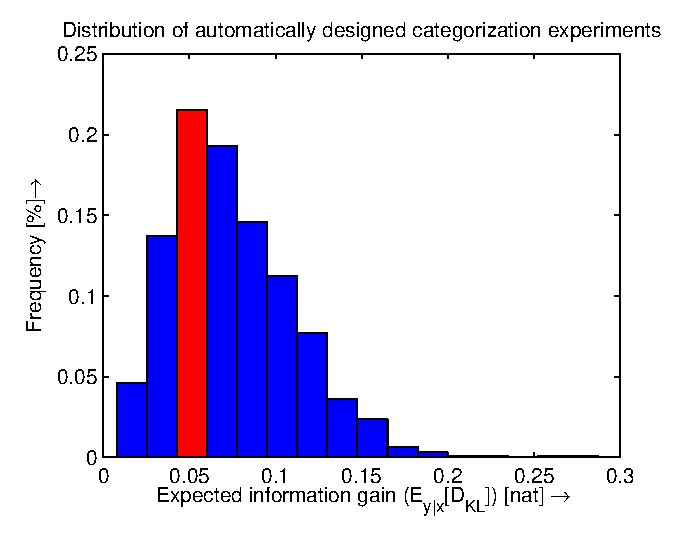
\includegraphics[width=3.2in]{img/dist.eps}
\caption{The distribution of optimal experiments with the MS bin highlighted in red.}
\label{fig:dist}
\end{figure}

The MS uses a qualitative swap in ranking for two stimuli to disambiguate the models. However, this prediction has a relatively small magnitude and comes at the expense of little information gain from the remaining stimuli. The optimal experiment is better able to quantitatively disambiguate the models by maximizing the information from all the stimuli simultaneously

The MS and optimal experiments were used to gather data from human participants on Mechanical Turk

The empirical results verify the OED predictions that the optimal experiment better disambiguates the two models (Fig.~\ref{fig:empirical})
\begin{figure}[h!]
\centering
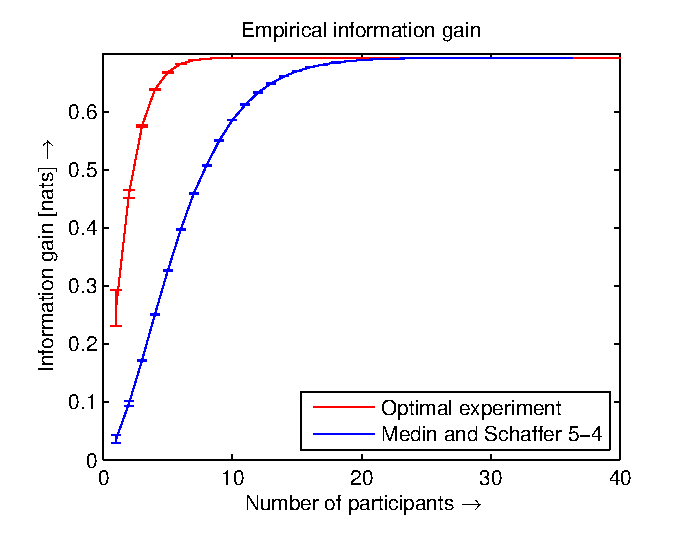
\includegraphics[width=3.2in]{img/empirical.eps}
\caption{Empirical information gain from $(n=40)$ Mechanical Turk participants. Error bars indicate standard error.}
\label{fig:empirical}
\end{figure}

%    \begin{itemize}
%        \item Overview
%            \begin{itemize}
%                \item This case study is based on Medin and Schaffer's (1978) work on disambiguating two models of classification learning~\cite{medin78:pr}
%                \item The purpose of this case study is to illustrate the efficacy of OED in psychology for the following scenarios:
%                    \begin{itemize}
%                        \item Discrete and non-ordinal experiment spaces
%                        \item Large combinatoric experiment spaces
%                        \item Parametric model classes
%                    \end{itemize}
%            \end{itemize}
%        \item Medin and Schaffer's theory of classification learning
%            \begin{itemize}
%                \item MS presented and contrasted two models of classification learning 
%                    \begin{enumerate}
%                        \item Context theory
%                            \begin{itemize}
%                                \item This is an exemplar model that classifies probe items by comparing similarities with retrieved instances of the category
%                                \item This is formalized as a statistical model that uses a sum of product computation to determine the probability a probe will be associated with a given category
%                            \end{itemize}
%                        \item Independent cue
%                            \begin{itemize}
%                                \item This is a prototype model that classifies probe items by comparing similarities with a representative prototype of the category
%                                \item This is formalized as a rank-ordering model that uses an additive computation to determine the relative association with a given category
%                                \item To convert this rank-ordering model into a statistical one, we use a log-linear transformation to convert the relative associations into probabilities
%                            \end{itemize}
%                    \end{enumerate}
%                \item These models are formalized in the probabilistic programming language Church
%                \item With meticulous forethought, MS designed an experiment to disambiguate these two candidate models and then analyzed participant's performance on using this prompt
%            \end{itemize}
%        \item Optimal experiment design
%            \begin{itemize}
%                \item Although MS provide sound arguments for their experiment design, does their experiment provide the optimal amount of information for disambiguating their competing models?
%                \item Constrained to the same MS experiment space, we exhaustively evaluated the 933 valid and unique experiments in terms of expected information gain
%            \end{itemize}
%        \item Results and discussion
%            \begin{itemize}
%                \item MS is a suboptimal experiment that ranks in the 30$^\text{th}$ percentile with respect to expected information gain (Fig.~\ref{fig:dist})
%\begin{figure}[h!]
%\centering
%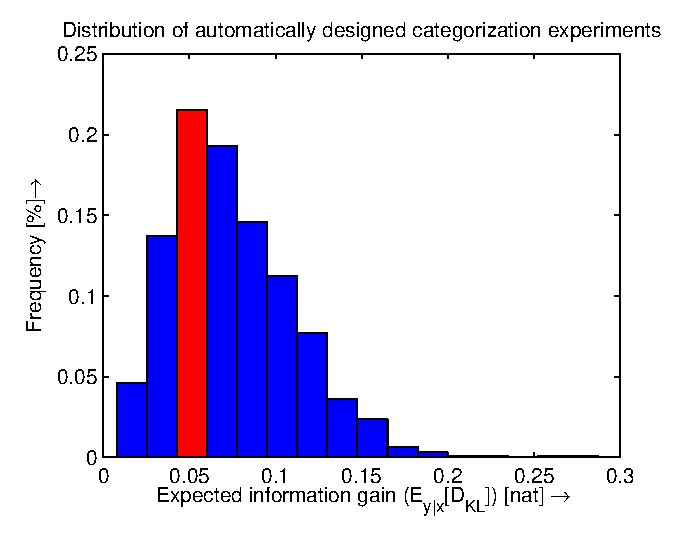
\includegraphics[width=3.2in]{img/dist.eps}
%\caption{The distribution of optimal experiments with the MS bin highlighted in red.}
%\label{fig:dist}
%\end{figure}
%                \item The MS uses a qualitative swap in ranking for two stimuli to disambiguate the models. However, this prediction has a relatively small magnitude and comes at the expense of little information gain from the remaining stimuli. The optimal experiment is better able to quantitatively disambiguate the models by maximizing the information from all the stimuli simultaneously
%                \item The MS and optimal experiments were used to gather data from human participants on Mechanical Turk
%                \item The empirical results verify the OED predictions that the optimal experiment better disambiguates the two models (Fig.~\ref{fig:empirical})
%\begin{figure}[h!]
%\centering
%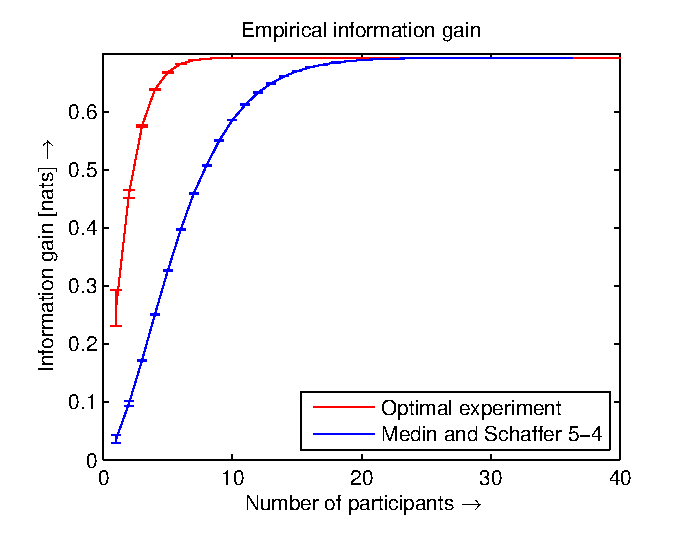
\includegraphics[width=3.2in]{img/empirical.eps}
%\caption{Empirical information gain from $(n=40)$ Mechanical Turk participants. Error bars indicate standard error.}
%\label{fig:empirical}
%\end{figure}
%            \end{itemize}
%        \end{itemize}
%
%\section{Case study 3: OED with model parameterization}
%    \begin{itemize}
%        \item Overview
%            \begin{itemize}
%                \item This case study is an extension of case study 2
%                \item The purpose of this case study is to illustrate the following scenarios:
%                    \begin{itemize}
%                        \item The use of OED for iterative model refinement
%                        \item The distinction between parameters that define distinct model hypothesis and  parameters within a class of models 
%                    \end{itemize}
%            \end{itemize}
%        \item Mathematical framework %\label{s:class:ss:math}
%            \begin{itemize}
%                \item Show framework with theta
%            \end{itemize}
%        \item Categorization models with inference
%            \begin{itemize}
%                \item A natural extension to MS's work is to question whether people are jointly inferring the parameters that define each category as well as the categories of stimuli 
%                    \begin{itemize}
%                        \item This example helps illustrate how OED can help guide the iterative design of new models
%                    \end{itemize}
%                \item We present an extension of both the context theory and independent cue models, where the model parameters are jointly inferred conditioned on successful recall tasks
%                \item \emph{Include: brief mathematical overview of normalizing over model parameters}
%                \item The resulting four different models can then be organized to into three distinct psychological hypotheses:
%                    \begin{enumerate}
%                        \item Which model best represents human categorization?
%                            \begin{itemize}
%                                \item Each of the four models is treated as a separate hypothesis
%                            \end{itemize}
%                        \item Are humans doing parameter inference in the categorization task?
%                            \begin{itemize}
%                                \item There are two classes of model hypotheses: models with and without inference
%                                \item Each model class is a hierarchical mixture model that combines the predictions of the inference and non-inference models, respectively
%                            \end{itemize}
%                        \item Are humans following either the context theory or independent cue models, regardless of their ability to infer model parameters?
%                            \begin{itemize}
%                                \item There are two classes of model hypotheses: context theory and independent cue
%                                \item Each model class is a hierarchical mixture model that combines the predictions of both the inference and non-inference models for their respective classification model
%                            \end{itemize}
%                    \end{enumerate}
%            \end{itemize}
%        \item Optimal experiment design
%            \begin{itemize}
%                \item Does the optimal experiment depend on the different psychological hypotheses?
%                \item We constrained the experiment space to the 933 experiments of case study 2 and evaluated the information gain for all three hypothesis
%            \end{itemize}
%        \item Results and discussion
%            \begin{itemize}
%                \item The optimal experiment does dependent on the psychological hypothesis
%                    \begin{itemize}
%                        \item The optimal experiment for hypothesis 1 and 2 are the same
%                        \item The optimal experiment for hypothesis 3 is the same as the case study 2
%                        \item It is not surprising that hypothesis 3 and case study 2 share the same optimal experiment as they share the same base model and the inference component creates a relatively small perturbation in the distributions
%                        \item It expected that hypothesis 2 has a separate optimal experiment as it differentiating a fundamentally different class of models
%                        \item Both the optimal experiments for hypothesis 2 and 3 are relatively informative for hypothesis 1, which treats each model as a separate psychological hypothesis. However, since the inference models produce more extreme predictions than their base counterparts, the hypothesis 2 optimal experiment best disambiguates the models
%                    \end{itemize}
%                \item \emph{Include: Statistics summarizing the rank ordering between the optimal experiments}
%                \item \emph{Include: Plots of the optimal experiments}
%                \item \emph{In progress (optional): Gather mechanical turk data?}
%                \item This case study illustrates the need to explicitly consider the psychological hypothesis when implementing OED
%                \begin{itemize}
%                    \item In turn, parameters within each hypothesis can be normalized with either a uniform or informative prior
%                \end{itemize}
%            \end{itemize}
%    \end{itemize}

\section{Case study 4: OED with respect to the number of participants}
    \begin{itemize}
        \item Overview
            \begin{itemize}
                \item The purpose of this case study is to provide an analysis for designing experiments that consider the number of participants
            \end{itemize}
        \item Mathematical theory %\label{s:npart:ss:math}
            \begin{itemize}
                \item To compute the information gain for a number of participants, $n_{ss}$, we compute the posterior using the joint observations $p(m|y_{1,x}, \dots, y_{n_{ss},x})$, where ${Y_{1,x}, \dots, Y_{n_{ss},x}}$ are i.i.d., and follow the established method
                \item This method has a number of properties:
                    \begin{enumerate}
                        \item Degenerate information gain
                            \begin{itemize}
                                \item $ I(M;Y_{x}) = 0 \text{ iff } p(y_x|m_0) = \dots = p(y_x|m_{n_m}),  \forall y$
                                \item There is zero information gain for only experiments with identical response distributions
                            \end{itemize}
                        \item Information gain is monotonic with respect to the number of participants
                            \begin{itemize}
                                \item $\forall M, Y, x: I(M;Y_{1,x}, \dots, Y_{n_{ss}-1,x}) \leq I(M;Y_{1,x}, \dots, Y_{n_{ss},x})$
                                \item It is impossible to lose information by increasing the number of participants 
                            \end{itemize}
                        \item Information gain is bounded and approached as the number of participants approaches infinity
                            \begin{itemize}
                                \item $\lim_{n \rightarrow \infty} I(M;Y_{1,x}, \dots, Y_{n_{ss},x}) = H(M)$
                                \item There is a limit to the information gain from adding additional participants 
                            \end{itemize}
                        \item The information gain is not guaranteed to be order-preserving with respect to the number of participants
                            \begin{itemize}
                                \item The optimal experiment depends on the number of participants
                                \item \emph{In progress: proof for order-preservation for 2 models}
                                \item \emph{Include: counter example to order-preservation for $n_m > 2$ models}
                            \end{itemize}
                    \end{enumerate}
                \item Note these properties only hold for expected information gain and not empirical information gain
                    \begin{itemize}
                        \item the assumption that one of the candidate models is the ground truth may not hold in empirical settings
                        \item \emph{In progress: Information gain for quantified divergence between empirical and theoretical settings}
                    \end{itemize}
                \item Computing the information gain for a number of participants is exponential: $O({n_y}^{n_{ss}})$, where $n_y$ is the size of the response space
                \item Approximating information gain using multinomial Monte Carlo sampling
                    \begin{itemize}
                        \item The response space is treated as the base distribution for a multinomial distribution and is sampled using Monte Carlo methods
                        \item \emph{Include: proof that a sum of random variables transform preserves mutual information for iid distributions}
                        \item According to the multivariate central limit theorem, the multinomial distribution approximates a multivariate Gaussian as the number of participants approaches infinity
                        \item As Gaussians are short tailed distributions, the frequency counts of the Monte Carlo method can be efficiently stored in memory using sparse coding data structures, such as hash tables
                        \item This approach is guaranteed to be asymptotically convergent with respect to the number of particles
                        \item The primary issue with this approach is that it requires design decisions with respect to the number of particles, which can affect accuracy, computational efficiency, and memory resources
                        \item \emph{In progress (optional): Computational complexity/memory utilization discussion?}
                    \end{itemize}
            \end{itemize}
        \item Models of social cognition
            \begin{itemize}
                \item This case study is based on D Hawthorne's work on how people integrate direct observations with social information
                \item An example of this context is a betting game where one's bet relies on estimating a winning probability with two independent streams of data
                    \begin{enumerate}
                        \item Direct observations -- one sees the outcomes of a number of trials
                        \item Social information -- one sees the bet placed by a neighboring actor along with the number of independent trials he observed, but not the outcome of those trials
                    \end{enumerate}
                \item We compare three different models of social cognition
                    \begin{enumerate}
                        \item Direct only -- the participant infers the winning probability based only on the direct observations
                        \item Social only -- the participant infers the winning probability based only on the social information
                        \item Integrative -- the participant infers the winning probability by integrating both streams of information in a Bayesian fashion
                    \end{enumerate}
            \end{itemize}
        \item Optimal experiment design
            \begin{itemize}
                \item The experiment design space is parameterized by three parameters (the actor always bets):
                    \begin{enumerate} 
                        \item The number of trials the actor observed
                        \item The number of trials the participant observes
                        \item The number of victories the participant observes
                    \end{enumerate}
                \item The model relies on one non-informative prior, the reliability of the actor, which was measured empirically
            \end{itemize}
        \item Results and discussion
            \begin{itemize}
                \item The optimal experiment varies depending on the number of participants (Fig.~\ref{fig:npart})
\begin{figure}[h!]
\centering
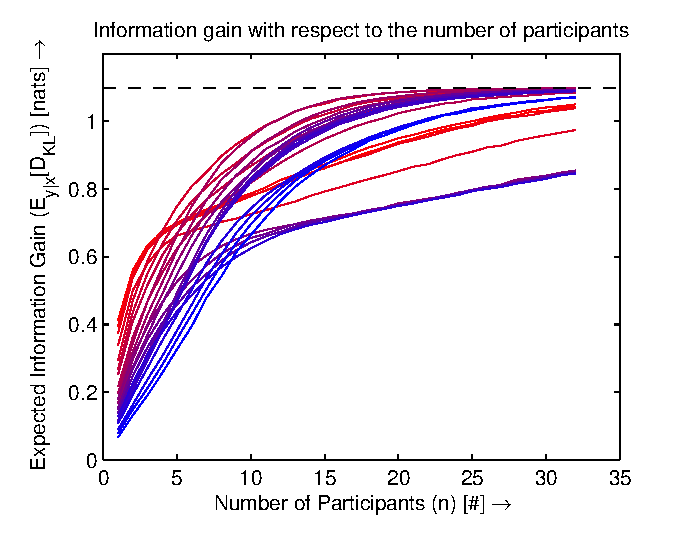
\includegraphics[width=3.2in]{img/npart.eps}
\caption{Theoretical information gain depending on the number of participants.}
\label{fig:npart}
\end{figure}
                    \begin{itemize}
                        \item Each line in Fig.~\ref{fig:npart} denotes the information gain of a single experiment parameter set; the color gradient is used to denote the ranking of the experiments from highest to lowest information gain with one participant using red and blue, respectively
                        \item There are a handful of experiments that provide high information gain for a small number of participants, but do not scale well with more participants
                            \begin{enumerate}
                                \item This is achieved by maximally differentiating the pair of direct only and integrative models with the social model
                                \item For a small number of participants, it rules out one of the sets of models. However, for a large number of participants, it is less effective at differentiating between the integrative and direct only models
                                \item \emph{Include: plots of the model distributions}
                            \end{enumerate}
                        \item Ultimately, the optimal experiments for a significant number of participants are suboptimal for a small number of participants, but scales better with more participants
                            \begin{enumerate}
                                \item For the optimal experiments, the modes of the distributions are less distinguished as a triplet, but more participants provides better estimates of these distributions and thus greater information gain with more participants
                                \item \emph{Include: plots of the model distributions}
                            \end{enumerate}
                    \end{itemize}

                \item Computational complexity (Fig.~\ref{fig:comp}
\begin{figure}[h!]
\centering
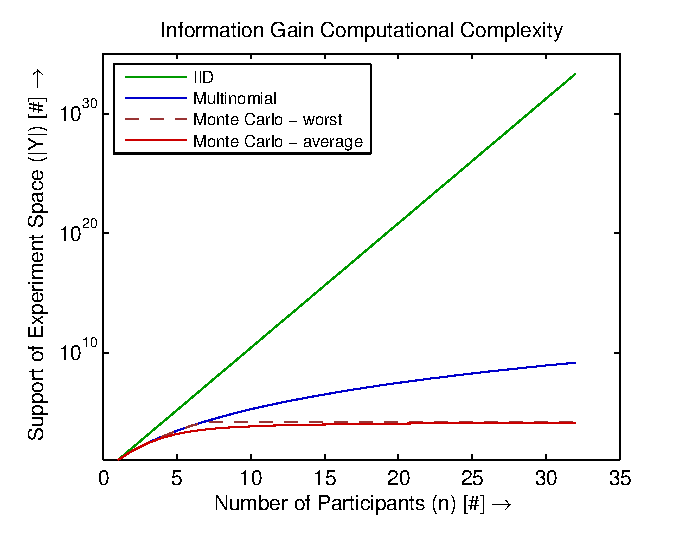
\includegraphics[width=3.2in]{img/comp.eps}
\caption{Theoretical information gain depending on the number of participants.}
\label{fig:comp}
\end{figure}
                    \begin{itemize}
                        \item Fig.~\ref{fig:comp} illustrates the computational efficiency of our multinomial Monte Carlo samping approach
                        \item IID is the distribution that results from taking each participant as an identical and independent sample from a distribution; the support of the space grows exponentially with respect to the number of participants
                        \item Multinomial is the distribution that results from taking the sum of the iid variables, transforming the distribution into a multinomial distribution; the support of the space grows factorially with respect to the number of participants
                        \item Monte Carlo is the distribution that results from approximating the multinomial distribution using a Monte Carlo sampling approach; the support of the space is bounded 
                        \item If the Monte Carlo sampling takes 1s of computational time, then for 32 participants, the multinomial distribution requires 27 hours and the IID distribution requires $4\times10^{21}$ years
                    \end{itemize}
            \end{itemize}
    \end{itemize}

\section{Case study 5: OED with dependent measures}
    \begin{itemize}
        \item Overview
            \begin{itemize}
                \item The purpose of this case study is to provide an analysis for experiment design with dependent measures
            \end{itemize}
        \item \emph{Todo}
    \end{itemize}

\section{Discussion and future work}

    \begin{itemize}
        \item This paper was focused on showing how to compute OED under a range of conditions. We did not focus on the search for optimal experiment design because we wanted to show how this approach is useful and we needed to dissociate that from the search process. In all the examples, we used exhaustive search that computed OED for all the problems. 
        \item This could be iterative. We skipped that too.
    \end{itemize}

\bibliographystyle{ieeetr}
\bibliography{oed}

\end{document}


